% mnras_template.tex
%
% LaTeX template for creating an MNRAS paper
%
% v3.0 released 14 May 2015
% (version numbers match those of mnras.cls)
%
% Copyright (C) Royal Astronomical Society 2015
% Authors:
% Keith T. Smith (Royal Astronomical Society)

% Change log
%
% v3.0 May 2015
%    Renamed to match the new package name
%    Version number matches mnras.cls
%    A few minor tweaks to wording
% v1.0 September 2013
%    Beta testing only - never publicly released
%    First version: a simple (ish) template for creating an MNRAS paper

%%%%%%%%%%%%%%%%%%%%%%%%%%%%%%%%%%%%%%%%%%%%%%%%%%
% Basic setup. Most papers should leave these options alone.
\documentclass[a4paper,fleqn,usenatbib]{mnras}

% MNRAS is set in Times font. If you don't have this installed (most LaTeX
% installations will be fine) or prefer the old Computer Modern fonts, comment
% out the following line
%\usepackage{newtxtext,newtxmath}
% Depending on your LaTeX fonts installation, you might get better results with one of these:
%\usepackage{mathptmx}
%\usepackage{txfonts}

% Use vector fonts, so it zooms properly in on-screen viewing software
% Don't change these lines unless you know what you are doing
\usepackage[T1]{fontenc}
\usepackage{ae,aecompl}



%%%%% AUTHORS - PLACE YOUR OWN PACKAGES HERE %%%%%

% Only include extra packages if you really need them. Common packages are:
\usepackage{graphicx}	% Including figure files
\usepackage{amsmath}	% Advanced maths commands
\usepackage{amssymb}	% Extra maths symbols
\usepackage[latin1]{inputenc}
\usepackage{tikz}
\usetikzlibrary{shapes,arrows}

%%%%%%%%%%%%%%%%%%%%%%%%%%%%%%%%%%%%%%%%%%%%%%%%%%

%%%%% AUTHORS - PLACE YOUR OWN COMMANDS HERE %%%%%

% Please keep new commands to a minimum, and use \newcommand not \def to avoid
% overwriting existing commands. Example:
%\newcommand{\pcm}{\,cm$^{-2}$}	% per cm-squared

%%%%%%%%%%%%%%%%%%%%%%%%%%%%%%%%%%%%%%%%%%%%%%%%%%

%%%%%%%%%%%%%%%%%%% TITLE PAGE %%%%%%%%%%%%%%%%%%%

% Title of the paper, and the short title which is used in the headers.
% Keep the title short and informative.
\title[]{Efficiently sampling rare events in population synthesis models}

% The list of authors, and the short list which is used in the headers.
% If you need two or more lines of authors, add an extra line using \newauthor
\author[]{Floor Broekgaarden et al. ,$^{1,2}$\thanks{E-mail: fsbroekgaarden@gmail.com}
(TBD)
%Stephen Justham,$^{1,2}$
%Ilya Mandel$^{1,3}$
%Jonathan Gair$^{1,4}$ \newauthor
%Tassos Fragos$^{1,5}$
\\
% List of institutions
$^{1}$Dark Cosmology Centre, Niels Bohr Institute, University of
Copenhagen, Juliane Maries Vej 30, DK-2100, K\o benhaven \o,
Denmark\\
$^{2}$ Astronomical Institute Anton Pannekoek, University of Amsterdam, P.O. Box 94249, 1090 GE, Amsterdam, The Netherlands \\
%$^{2}$Kavli Institute for Astronomy and Astrophysics, Peking University,
%Beijing, China\\
%$^{3}$School of Physics and Astronomy, University of Birmingham, Birmingham B15 2TT, UK\\
%$^{4}$School of Mathematics, University of Edinburgh, The King`s Buildings, Peter
%Guthrie Tait Road, Edinburgh, EH9 3FD, UK
% \\
%$^{5}$Geneva Observatory, University of Geneva, Chemin des Maillettes 51,
%1290 Sauverny, Switzerland
}

% These dates will be filled out by the publisher
%\date{Accepted XXX. Received YYY; in original form ZZZ}

% Enter the current year, for the copyright statements etc.
\pubyear{2018}

% Don't change these lines
\begin{document}
\label{firstpage}
\pagerange{\pageref{firstpage}--\pageref{lastpage}}
\maketitle

% Abstract of the paper
\begin{abstract}

\end{abstract}

% Select between one and six entries from the list of approved keywords.
% Don't make up new ones.
\begin{keywords}
importance sampling -- population synthesis -- gravitational waves
\end{keywords}

%%%%%%%%%%%%%%%%%%%%%%%%%%%%%%%%%%%%%%%%%%%%%%%%%%

%%%%%%%%%%%%%%%%% BODY OF PAPER %%%%%%%%%%%%%%%%%%







\section{Introduction}
\label{sec:introduction}
%
\begin{itemize}
\item introduce problem
\item binary black holes BBH , LIGO
\end{itemize}
%

\section{Binary population synthesis}
\label{sec:BPS}
Binary population synthesis models are a versatile tool in astrophysics to make predictions for populations of stars and the rate of astrophysical transient events of stellar origin. 
The models include a large variety of physical processes that can take place during the evolution of a star in a binary system such as super nova explosions, stellar winds, mass transfer and common envelope evolution. Examples of binary population synthesis models are  BSE \citep{hurley2000comprehensive,hurley2002evolution}, binary$\_$c \citep{izzard2004new, izzard2009population}, StarTrack \citep{belczynski2008compact}, SEBA \citep{portegies1996population,verbunt1996high} (\textbf{also add Portegies-zwart $\&$ Yungelson 1998 and Nelemans 2011??}), COMPAS \citep{stevenson2017formation} and ComBinE (Kruckow, submitted 2018). These models interpolate between evolutionary tracks of single stars obtained with a detailed stellar structure code \citep{pols1998stellar} and rely on an approximate treatment of the physical processes.  By doing so, they present a rapid code that can compute the evolution of many stars within a simulation. 
Binary population synthesis models have now been used to study a variety of astrophysical problems ranging from the characteristics of young stellar populations and how they are affected by the products of binary interaction \citep{de2013rotation,schneider2014bonnsai}  to the end stages as core collapse supernova \citep{zapartas2017delay}, and the more exotic outcomes such as type IA supernovae \citep{toonen2012supernova}, and gravitational wave sources \citep{belczynski2017gw170104}.

Since it is not known a priori which part of the initial parameter space produces a certain binary population of interest, the parameter space needs to be explored. This is generally done  by drawing many samples, i.e. binary systems $\mathbf{x_i}$, of initial binary parameters and evaluating them with the BPS model into their final state $\mathbf{x_f}$,  
%
\begin{equation}
	\mathbf{x_f} = u(\mathbf{x_i}),
	\label{eq:BPS-u(x)}
\end{equation}
%
where $u$ here represents the BPS model evaluation.

Often, BPS models are used to study a population of binaries of a certain subtype $\mathbf{X_t}$, e.g. BBHs, and therefore it is  useful to define a function, 
%
 \begin{align*}
 \phi(\mathbf{x_f} | \mathbf{x_i}, u) = \begin{cases}    1 \ \ \text{if } \mathbf{ x_f} \in   \mathbf{X_t}    \\ 0 \ \   \text{else,}   \end{cases}
 \end{align*} 
% 
that equals unity if $\mathbf{x_i}$ evaluated to the target binary system $\mathbf{X_t}$ and zero if not.  
We will use this function throughout the paper as it is the main objective to perform the inference on. 

The adaptive importance sampling method introduced in this paper can be applied to many different (BPS) codes. 
In the next section,  however, we will introduce the BPS code COMPAS and our settings for the code that is used throughout this paper to demonstrate the strengths of this method. 
% 
%\begin{itemize}
%\item BPS are rapid stellar evolution codes based on Hurley and Pols that 
%\item introduction to BPS and examples of codes, and papers in which BPS is used (SEBA, COMPAS, CombIned,... )
%\item we will use COMPAS throughout this paper
%\item BPS are basically functions that evaluate a set of initial conditions and output a set of final stars. 
%\end{itemize}
%%
%
%
\subsection{Physics in COMPAS}
\label{subsec:physicsCOMPAS}
%
Compact Object Mergers: Population Astrophysics and Statistics (COMPAS), is a BPS code that focuses on GW astrophysics and in particularly is designed to study uncertainties in binary evolution and  compact mergers that possibly form the GW progenitors  and optimize the information that can be obtained from simulations \citep{barrett2017accuracy}. In this work the code is used to analyse binary black holes that merge within Hubble time and therefore form potential progenitors for the observed GWs by the LIGO and VIRGO collaboration. The COMPAS model includes the so-called `isolated binary evolution channel' for BBH mergers, where both stars initially start with a large separation and thus evolve separately and often a \emph{`commen envelope'} phase is needed to bring the stars closer together such that they can merge within Hubble time. Details of this channel are given in \citep{belczynski2016first}.   

Like most BPS codes, COMPAS includes many physical processes such as common envelope, mass transfer and kick velocity prescriptions. Throughout this paper we employ the \citep{stevenson2017formation} fiducial model. 
Some exceptions on the fiducial model are described below. 

\begin{itemize}
	\item Metallicity, The metallicity of all simulations is set to $Z = 0.00X Z_{\odot}$, which represent the low metallicity environment where massive black holes can be born. 
	\item We focus on BBH mergers that merge within Hubble time. Our target distribution $\mathbf{X_t}$ therefore consists of these binaries that evolve to two black holes. Furthermore we only select  the binaries that did not have roche-lobe overflow after the commen envelople phase \textbf{(say something about optimistic / pessimistic?? )}. 
	\item (add other differences with Stevenson+17 and COMPAS settings I have)
\end{itemize}


\subsection{Initial parameter priors}
\label{subsec:priorsCOMPAS}
Since the details of binary evolution are uncertain, a large number of binaries is simulated with BPS models to thoroughly explore the space of initial conditions. The uncertainties are then captured in tunable parameters $\mathbf{x}$  which distribution functions are observably derived. Often between 3 and 20 parameters are used in BPS but for the purpose of this paper we will focus on the three most important variables: the initial mass of the primary star (i.e., the most massive star) $M_{1,i}$, the mass ratio, $q_i = M_{1,i} / M_{2,i}$, between the two stars and  the initial separation, $a_i$. Each initial binary sample can thus be represented by three parameter values
%
\begin{equation}
	\mathbf{x_i} = (M_{1,i},\ a_i, \ q_i). 
\end{equation}
%
The reason that we focus on these three parameters is (i) because above parameters are the most important  parameters in the sense that they dominate the outcome and thereby the uncertainty of the evolution (ref Belczynski $\&$ Selma or Moe?) , and (ii) that especially the primary mass and separation have an extremely steep distribution function which can drastically increase the computational costs when simulating rare events (see Section \ref{sec:aplication-I}).  The distribution functions used in this paper for the three parameters are given below. 
Although only a subsection of three parameters are used in this work,   the adaptive importance sampling method can straightforwardly be extended to all initial parameters. 


\subsubsection{Primary mass $M_{1,i}$}


The distribution of the initial primary mass $M_1$ follows a power law distribution 
also known as the initial mass function (IMF) \citep{kroupa2001variation}:
%
\begin{equation}
    p(M_{1,i}) = K_M M_{1,i}^{-\alpha},  \ M_{1,i} \in [M_{1,i, \text{min}} , M_{1,i, \text{max}} ], 
\label{eq:prior-IMF}
\end{equation} 
%
where  $K_M$ is the normalization constant given by
%
\begin{equation*}
	K_M - \frac{\alpha + 1}{M_{1, \text{max}}^{\alpha +1 } -  M_{1, \text{min}}^{\alpha +1 }}. 
\end{equation*}
%
We choose $\alpha = 2.35$ and the primary mass to be in the range $M_{1,i} \in [7,100] M_{\odot}$, consistent with \citep{stevenson2017formation}.  \\
%
%
\subsubsection{Mass ratio $q_i$}
%
The mass ratio $q_i$ is suggested from observations to have a flat distribution (Mazeh et al., 1992; Goldberg $\&$ Mazeh, 1994; Tout, 1991),  given by
%
\begin{equation}
    p(q_i) =  \frac{1}{q_{ \text{max}} - q_{ \text{min}}}  , \ q_i \in (q_{ \text{min}}, q_{ \text{max}}],  
	\label{eq:prior-massratio}
\end{equation}
%
where $(q_{ \text{min}}, q_{ \text{max}}] = (0,1]$ by definition of $q$. 
Nevertheless, it is also suggested that there is some dependency of the mass ratio on the period of the
system (e.g. Moe $\&$ Di Stefano 2016).
%
\subsubsection{Separation $a_i$}
The separation $a_i$ is found to be uniform in log, also known as Opiks law \citep{opik1924statistical} and consistent with findings by \citep{kobulnicky2014toward} and \citep{moe2015early}.  The distribution function is given by
%
\begin{equation}
    p(a_i) = \frac{K_a }{a_i},   \ a_i \in [a_{\text{min}} , a_{\text{max}} ],
	\label{eq:prior-separation}
\end{equation} 
%
where $K_a$ is the normalization constant.
%
\begin{equation*}
	K_a = \frac{1}{\log a_{\text{max}}- \log a_{\text{min}}} 	
\end{equation*}
%
We choose $[a_{\text{min}} , a_{\text{max}} ] =  [0.1,10^3]$  AU consistent with \citep{stevenson2017formation}. 





Assuming the parameters $M_{1,i}, q_i, a_i$ to be independent the combined prior distribution of $\mathbf{x_i}$ then becomes:
%
\begin{equation}
	p(\mathbf{x_i}) = p({M_{1,i}}) \ p({a_i}) \  p({q_i}).
	\label{eq:prior-3d}
\end{equation} 
%
These distributions can now be used to model a population of stars using sampling methods. 
%


\section{Sampling methods}
\label{sec:sampling-methods}
In general BPS, a large number of binaries $\mathbf{x_i}$ are drawn from their birth distribution (Eq. \ref{eq:prior-3d}) either (i) randomly,  in which case the statistics of the targeted population are estimated using the Monte Carlo estimator  or (ii) by creating a uniform grid in parameter space and weighing each sample grid point with the birth distribution. 
Examples of BPS models that use random draws via Monte Carlo sampling are StarTrack, COMPAS and SEBA, whilst binary$\_$c and ComBinE use grid based sampling \textbf{(DOUBLE CHECK THIS)}.
In both sampling strategies, simulating rare events (e.g. BBH mergers) becomes computationally expensive and often an intractable problem as a large part of the simulations are spend on evaluating initial binary systems $\mathbf{x_i}$ that don't evolve to a binary system of the target population. In this section we therefore introduce an adaptive importance sampling method that reduces the costs of simulating rare events with BPS by introducing a sampling scheme that aims to adaptively change the sampling distribution towards the target distribution. 



 


%
%
%\subsection{Monte Carlo sampling}
%\label{subsec:MCsampling}
%%
%In monte carlo random sampling
%%
%
%
%\subsection{Uniform grid sampling}
%\label{subsec:UNIsampling}
%%
%In uniform grid
%%

\subsection{Adaptive importance sampling}
\label{subsec:AISsampling}
%



The adaptive importance sampling (AIS) method consists of three main steps which are schematically shown in Fig. \ref{fig:aIS_scheme}. 
\begin{enumerate}
	\item First, there is a so-called  \emph{exploratory phase}     since it is not known a priori which part of the parameter space produces binaries of the type that is contained in the target distribution. In this phase initial samples are drawn from their birth distribution  either randomly or by creating a regular grid (uniform method) and evaluated in the model until a certain number $N_{\text{E,t}}$  of  binaries of the target type $\mathbf{X_t}$ are found. I.e. the sampling continues until  there is a set of $N_{\text{E,t}}$ binaries of the target simulation $\mathbf{x_f} \in  \mathbf{X_t}$. The choice of $N_{\text{E,t}}$ depends mostly on the aimed sampling uncertainty of the simulation and is explained further in Section \ref{subsec:standard-AIS}. 
	\item Secondly, a new sampling distribution, $g(\mathbf{x}) $, the so-called \emph{instrumental distribution} is defined by drawing Gaussian distributions in the initial parameter space around each of the $N_{\text{E,t}}$ `successful' binaries $x_{E,k} $ with $k = 1, ..., N_{\text{E,t}}$ that evaluated to a binary system of the target population.  The instrumental distribution $g(\mathbf{x})$ is thus given by the Gaussian mixture distribution:
	%
	\begin{equation}
	    g(\mathbf{x}) = \sum _{k=1}^{N_{\text{E,t}}}  g_k(\mathbf{x}) w_k =   \sum _{k=1}^{N_{\text{E,t}}}  \mathcal{N}({\boldsymbol {\mathbf{x_{t,k}},\Sigma_{k}}}) w_k 
	\label{eq:instrumental-distribution}
	\end{equation}	 
	%	
	where each $\mathcal{N}({\boldsymbol {\mathbf{x_{t,k}},\Sigma _{k}}})$ is a multivariate Gaussian distribution with mean $\mathbf{x_{E,k}}$ and covariance matrix $\mathbf{\Sigma _{k}}$. Furthermore, $w_k$ are the weights of each Gaussian distribution, which equals the weight of drawing the initial sample $x_i$ ($w_k = 1$ in the Monte Carlo random drawing). 
	
	\item Thirdly, new samples are now drawn from the instrumental distribution $g(\mathbf{x}) $ and evaluated with the BPS model.  Assuming the  outcome function $\phi(\mathbf{x_i})$ to be locally continuous (and not chaotic), a larger fraction of the samples will now produce binaries of the target distribution, and as a result, the simulation will model the target distribution more efficient. 
\end{enumerate}
After a certain number of draws, step (ii) and step (iii) can be repeated to even more increase the efficiency. 
%
\begin{figure}
	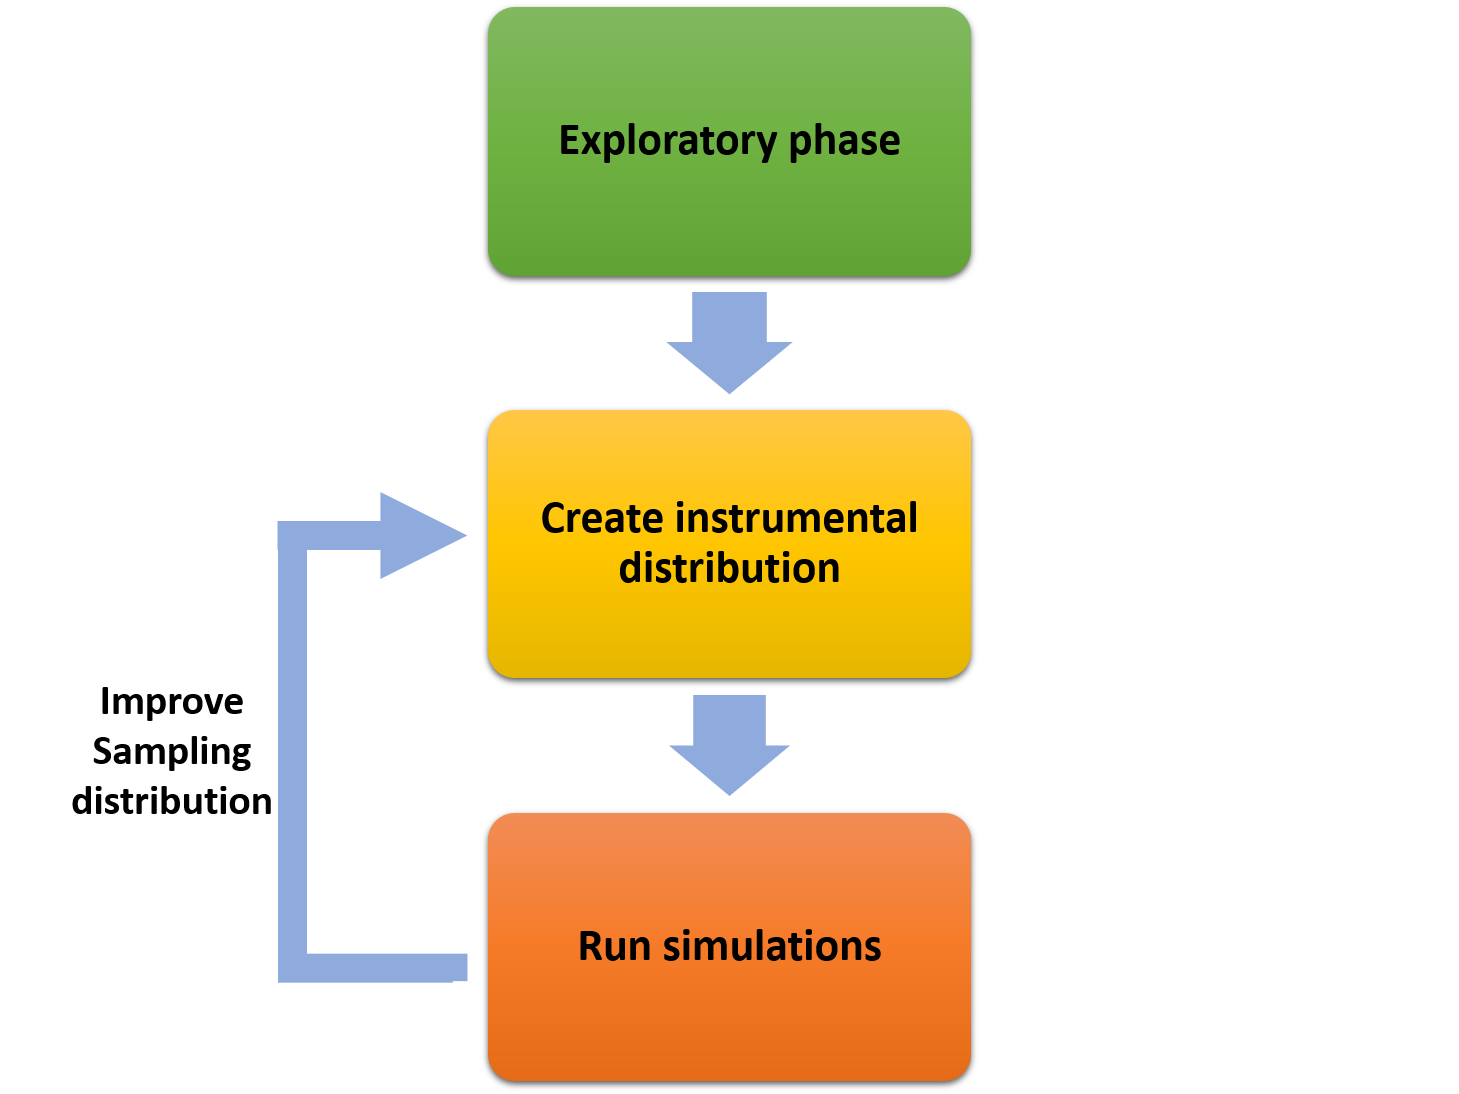
\includegraphics[width=\columnwidth]{flowchartAISv2.png}
    \caption{Flowchart of the adaptive importance sampling method that is used in this paper.  \textbf{should I add an input arrow with input priors and parameters and an output arrow for `inference'??}}
    \label{fig:aIS_scheme}
\end{figure}
%

At the end of a run, the statistics of the target distribution such as the expectation value of $\phi(x)$, i.e. its rate,  and  distribution functions can be determined by using the AIS estimator

\begin{equation}
	\widetilde{\mathbb{E}[\phi(\mathbf{x})]}_{N_t} = \frac{1}{N_t} \sum_{i=1}^{N_t} \phi(\mathbf{x_i}) \frac{p(\mathbf{x_i})}{g(\mathbf{x_i})}, 
	\label{eq:ISestimator}
\end{equation}
where $N_t$ is the total number of sample drawn from the instrumental distribution. \textbf{change this to multiple generations see notes other notebook}

In general, the AIS method is based on easy to implement steps. However, many choices on for example the covariance matrices, the exploratory sampling and other sampling strategies can be made to optimize the AIS method. Below we will therefore first introduce our \emph{`standard'} AIS method which is a minimal working implementation of the AIS method that is used throughout the paper and demonstrated in section \ref{sec:aplication-I} to already reduce the simulation costs. Of course many more adjustments can be made, some of which are discussed in Subsection \ref{subsec:var_standardAIS}.     


\subsubsection{Standard implementation}
In this subsection we will describe our so-called \emph{standard implementation} of AIS, which is used mostly throughout this paper. Although variations on this standard implementation might make the AIS method more efficient, we choose to first demonstrate the results with this more basic implementation of AIS to make it easier to understand the method and its strengths. Moreover, the choice of variations often varies for each simulation. A few examples of possible variations are discussed in the next section. 

\begin{enumerate}
	\item We choose $ N_{\text{E,t}} = 100 $ and an exploratory sampling using random draws from the birth distribution (Eq. \ref{eq:prior-3d}), i.e. Monte Carlo sampling.  We make this choice since Monte Carlo sampling produces samples with weights equal to unity, which  is the simplest sampling method for the exploratory phase of AIS. The choice of $ N_{\text{E,t}} = 100 $ implies that we will continue sampling random draws from the birth distribution until we have simulated $100$ initial binaries that evolved successfully to a target binary ($\mathbf{x_f} \in \mathbf{X_t}$). Since all samples have equal weight this implies that if we missed in our exploratory phase an area of the parameter space that also produces binaries of our target binary type, that this `missed island' most likely contributes less than $1/100$ to the total integral and thus statistics (such as the BBH fraction and/or the BBH merger rate ). 
	
	\item The instrumental distribution. Since we use random draws the weights $w_k$ in Eq. (\ref{eq:instrumental-distribution}) are equal to $ 1 / N_{\text{E,t}} $ and each Gaussian distribution contributes equally to the instrumental distribution. 
For simplicity, we  adopt a diagonal covariance matrix for $\Sigma$. Moreover, we scale the covariance matrix $\Sigma_k$  with the average expected distance locally between our initial sample points $ \mathbf{x_i}$ in the initial binary parameter space. This is chosen such that samples drawn from a Gaussian $\mathcal{N}({\boldsymbol {\mu _{i},\Sigma _{i}}})$  will generally fall in the space between the successful point  $x_i$ and its nearest neighbours.  Since the exploratory phase does not place the samples uniformly throughout the initial parameter space, e.g., many more binaries are created with low initial primary mass $M_{1,i}$ since low mass stars are much more common ( see  Eq. \ref{eq:prior-IMF}).
Therefore, we first transform the samples to a uniform sampled space, and then draw Gaussians around the space where it is uniform. This implies that the covariance matrix for the Gaussian distribution is given by

%
\begin{equation}
\Sigma_k = \begin{bmatrix} 
    \sigma_{1}^2 & 0 & \dots \\
    \vdots & \ddots & \\
    0 &        & \sigma_{d}^2 
    \end{bmatrix}, 
	\label{eq:covariance-matrix}
\end{equation}
%
where each $\sigma_{j,k} $  is given by
%
\begin{equation}
	\sigma_{j,k} =  \frac{\|p_j(x_{k, \text{max}})^{-1} - p_j(x_{k, \text{min}})^{-1} \|}{(N_{\text{E}})^{1/d}} \\
	  \text{ for } j = 1,.. ,\text{d}, k = 1, ... , N_{\text{E,t}} 
	\label{eq:sigma-covariance-matrix}
\end{equation}
%
where $p_j^{-1}$ is the inverse of the probability distribution function of the $j$-th parameter (see Subsection \ref{subsec:priorsCOMPAS}) and $N_E$ is the total number of simulations run for during the exploratory phase. 

	\item  \emph{Stopping criteria}. For the stopping criteria of the simulation we use for the standard AIS implementation to stop when a total number of $N_{\text{tot}} = XX $ samples have been evaluated. This represents the finite computational time that is often available for simulations due to scarce computational resources. Another possible stopping criteria could be defined by reaching a certain accuracy, this is further discussed in Subsection \ref{subsec:var_standardAIS}. 
	
\end{enumerate}

%\label{subsec:standard-AIS}
%\begin{itemize}
%	\item Exploratory sample
%	\item Refined sampling 
%	\item Estimators 
%	\item Stopping criteria := aimed accuracy (...) Performing inference on a finite number of simulations run induces an sampling error, this sampling error can be estimated    
%\end{itemize}
%


\subsubsection{Variations on the standard implementation}
\label{subsec:var_standardAIS}
\begin{itemize}
	\item multiple generations of $g$
	\item other ways of running exploratory run 
	\item fixed error
	\item stratified sampling 
	
\end{itemize}
%



\section{Application I}
\label{sec:aplication-I}

\subsection{More BBHs in simulation}
\label{subsec:AISsampling}
%
%
\begin{itemize}
\item 
\end{itemize}
%


\begin{figure}
	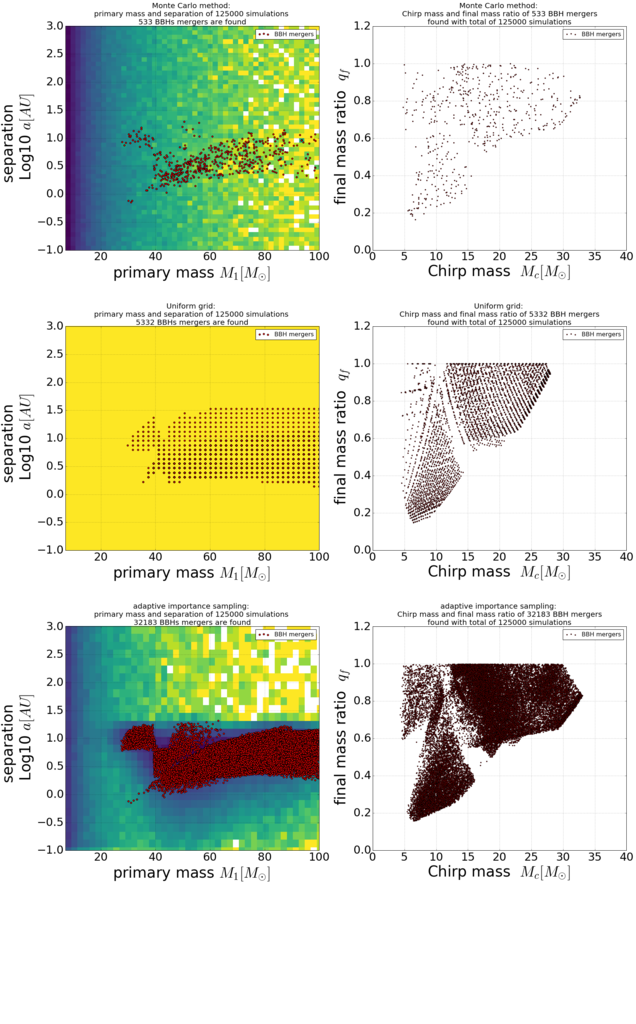
\includegraphics[width=\columnwidth]{bbhmergers_samplingmethods_plot_density_v2_1024.png}
    \caption{Example of   samples that are drawn (left)  uniformly distributed over the initial parameter space and (right) follow their birth distribution. The samples in the right plot are centred in the left corner since in the primary mass birth distribution used here low mass stars are much more common that high mass stars. }
    \label{fig:sampling_methods}
\end{figure}


\subsection{Rate estimator}
\label{subsec:RateI}
%
%
\begin{itemize}
\item 
\end{itemize}
%



\subsection{Chirp mass distribution}
\label{subsec:ChirpDistributionI}
%
%
\begin{itemize}
\item 
\end{itemize}
%


\section{Application II}
\label{sec:aplication-II}
%
\begin{itemize}
\item 
\end{itemize}
%


\section{(...)}


\section{Discussion}
\label{sec:discussion}
%
\begin{itemize}
\item 
\end{itemize}
%

\section{Summary }






\section*{Acknowledgements}

We thank the the Kavli Foundation, Niels Bohr institute and DARK Cosmology Centre in Copenhagen for their hospitality and for organising the Kavli summer school in gravitational waves astrophysics 2017. This work could not have been done without their support. 

%%%%%%%%%%%%%%%%%%%%%%%%%%%%%%%%%%%%%%%%%%%%%%%%%%

%%%%%%%%%%%%%%%%%%%% REFERENCES %%%%%%%%%%%%%%%%%%

% The best way to enter references is to use BibTeX:

\bibliographystyle{mnras}
\bibliography{my_bib} % if your bibtex file is called example.bib


% Alternatively you could enter them by hand, like this:
% This method is tedious and prone to error if you have lots of references
%\begin{thebibliography}{99}
%\bibitem[\protect\citeauthoryear{Author}{2012}]{Author2012}
%Author A.~N., 2013, Journal of Improbable Astronomy, 1, 1
%\bibitem[\protect\citeauthoryear{Others}{2013}]{Others2013}
%Others S., 2012, Journal of Interesting Stuff, 17, 198
%\end{thebibliography}

%%%%%%%%%%%%%%%%%%%%%%%%%%%%%%%%%%%%%%%%%%%%%%%%%%

%%%%%%%%%%%%%%%%% APPENDICES %%%%%%%%%%%%%%%%%%%%%

%\appendix

%\section{Some extra material}


%%%%%%%%%%%%%%%%%%%%%%%%%%%%%%%%%%%%%%%%%%%%%%%%%%


% Don't change these lines
\bsp	% typesetting comment
\label{lastpage}
\end{document}

% End of mnras_template.tex
